\section{衝撃波}
圧縮性流体になると音速が定義できる。音速よりも流速が速くなる場合には衝撃
波が発生する。

ある流速$\bm{u}$の中で、乱れが発生したとき、その乱れは圧縮性流体の場合は
音速で乱れが伝播する。これは音響近似が適用できる程度のに乱れの振幅が小さ
く、流速が小さい場合に適用できる。ここで、流速が大きくなった場合について
考える。乱れは流れに乗って移流していくので、乱れは流れに乗り、更に音速で
伝播していく。従って、乱れの放射する方向の単位ベクトルを$\bm{n}$とすると、
乱れの伝播速度は$\bm{u}+c\bm{n}$になる。

このとき、流速$\bm{u}$が音速よりも小さい場合には乱れはどの方向にも伝播し
ていくが、流速の方が早い場合には乱れの伝播する方向が限定される。そして、
図\ref{fig_shock}のような錐の範囲に超音速の場合の乱れの伝播範囲が限定さ
れる。すなわち、乱れの三角形の範囲の外側へは乱れは伝播しない。そして、そ
のなす角をMach数として、衝撃波の伝播範囲を表す。

\begin{figure}[htbp]
\begin{center}
 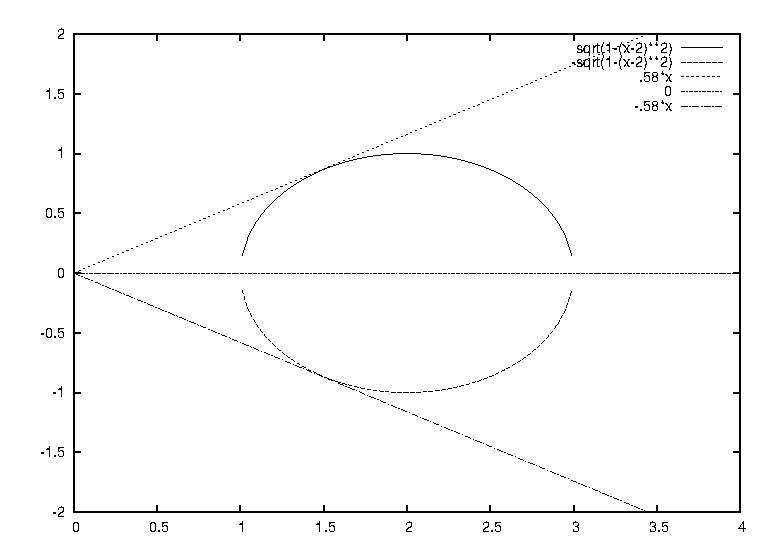
\includegraphics[width=450pt,height=450pt,angle=0]{shock.eps}
 \caption{衝撃波の伝播とMach角}
 \label{fig_shock}
 \end{center}
\end{figure}

\subsection{定常流の中の衝撃波}
最初に、定常的な流れの中の衝撃波について考える。圧縮性流体ではBernoulli
の定理が、
\begin{equation}
 h_0 = h + \frac{u^2}{2},
\end{equation}
で表される。

また、エントロピーは、エントロピーの保存則により、
\begin{equation}
 \bm{u}\cdot\text{grad}s = 0,
\end{equation}
である。そして、流れが一次源流の場合には$u ds/dl=0$なので、$s=Const.$で
ある。

圧縮性流体での質量流速は常に保存し、運動方程式とともに、
\begin{equation}
 j = \rho u,
\end{equation}
\begin{equation}
 \bm{u}\cdot\text{grad}\bm{u} = -\frac{1}{\rho}\text{grad}p,
\end{equation}
である。流線上では、運動方程式は、
\begin{equation}
 u\frac{du}{ds} = -\frac{1}{\rho}\frac{dp}{ds},
\end{equation}
となる。ここで、$s$はこの式でのみ弦長を表す。そして、これより、$udu =
-dp/\rho$が得られる。

ここで、音速の定義から$c^s = dp/d\rho$なので、$dp = c^2d\rho$で、
\begin{equation}
 d\rho u = 
  \rho\left(1-\frac{u^2}{c^2}\right),
\end{equation}
となる。この微分方程式から次のことがいえる。

\begin{enumerate}
 \item $1<u/c$の超音速のときは$d\rho u/du<0$であり、流速が大きくなると質
       量流束は小さくなり、流線が衝撃波から広がっていく
 \item $u/c<0$の亜音速のときは$0<d\rho u/du$であり、流速が大きくなると質
       量流束が大きくなり、流線が衝撃波へ集まっていく
 \item $u/c=1$のときには$d\rho u/du=0$で極大値を持つ
\end{enumerate}

このように流れの様子が亜音速から超音速へ遷移するときに大きく変わる。この
ように質量流束$j$が最大値$j_*$になる点での流速を臨界流速$u_*$と定義する。
そして、このとき$u=c$なので、$u_*=c$である。更にいえば、音速は圧力、密度
により変化する値なので、流速が変化にも影響を受ける。従って、臨界流速に対
応して、臨界音速$c_*$を定義できる。そして、このときにBernoulliの定理は、
\begin{equation}
 h_0 = h_* + \frac{c_*^2}{2},
\end{equation}
で表される。また、エントロピーも、
\begin{equation}
 s=s_*,
\end{equation}
である。そして、臨界音速は、
\begin{equation}
 c_* = c_0\sqrt{\frac{2}{\gamma - 1}},
\end{equation}
となる。

そして、熱力学の公式と、これら臨界流速のときの種々の熱力学関数の性質から、
臨界流速に達した際の圧縮性流体の性質を導くことができる。最初に、密度と、
圧力について、断熱圧縮の性質からもとめる。これは純粋に気体にだけ適用でき
る公式である。
\begin{equation}
 \rho = \rho_0
  \left(\frac{T}{T_0}\right)^{\frac{1}{\gamma - 1}},
\end{equation}
\begin{equation}
 p = p_0 \left(\frac{\rho}{\rho_0}\right)^{\gamma},
\end{equation}
が得られて、$c_PT=c^2/(\gamma - 1)$なので、これから、
\begin{equation}
 T_0 = T\left(1-\frac{\gamma - 1}{2}\frac{u^2}{c_0^2}\right)
  = T\left(1-\frac{\gamma - 1}{\gamma + 1}\frac{u^2}{c_*^2}\right),
\end{equation}
\begin{equation}
 \rho = 
  \rho_0 \left(
   1 - \frac{\gamma - 1}{2}\frac{u^2}{c_0^2}
  \right)^{\frac{1}{\gamma - 1}}
  = \rho_0 \left(
   1 - \frac{\gamma - 1}{\gamma + 1}\frac{u^2}{c_*^2}
	   \right)^{\frac{1}{\gamma - 1}},
\end{equation}
\begin{equation}
 p = p_0\left(
   1 - \frac{\gamma - 1}{2}\frac{u^2}{c_0^2}
\right)^{\frac{\gamma}{\gamma - 1}}
 = p_0\left(
   1 - \frac{\gamma - 1}{\gamma + 1}\frac{u^2}{c_*^2}
\right)^{\frac{\gamma}{\gamma - 1}}
\end{equation}
\begin{equation}
 u^2 = \frac{2c_0^2}{\gamma - 1}
  \left\{1-\left(\frac{p}{p_0}\right)^{\frac{\gamma - 1}{\gamma}}\right\}
  = \frac{2\gamma}{\gamma - 1}\frac{p_0}{\rho_0}
  \left\{1-\left(\frac{p}{p_0}\right)^{\frac{\gamma - 1}{\gamma}}\right\},
\end{equation}

\subsection{衝撃波断熱曲線}
衝撃波の一般的な性質、$p-V$曲線上での振る舞いについて考える。

最初に定常流について考える。一次元の定常流では、流速が空間的な保存量にな
る。それは衝撃波があるところ、ないところの区別なく成立するものなので、衝
撃波を挟んだ領域でも成立する。衝撃波の前縁を領域1、後縁を領域2とする。領
域1と領域2の間で各種流束は同じ値をとる。従って、
\begin{equation}
 \left[\rho u\right]^2_1 = 0, 
\end{equation}
\begin{equation}
 \left[\rho u^2 + p\right]^2_1 = 0,
\end{equation}
\begin{equation}
 \left[\rho u \left(h + \frac{u^2}{2}\right)\right]^2_1 = 0,
\end{equation}
となる。

ここで、質量流束を$j = \rho_2u_2 = \rho_1u_1$として定義すると、
\begin{equation}
 \rho_1u_1 = \rho_2u_2 = j,
\end{equation}
である。

次に、体積を比体積として、$V_1 = 1/\rho_1$、$V_2 = 1/\rho_2$と定義する。
このとき、質量流束と運動量流束の保存則から、
\begin{equation}
 u_1 = j V_1,\mspace{20mu}
  u_2 = j V_2,
\end{equation}
\begin{equation}
 p_1 + \rho_1 j^2 V_1^2 = p_2 + j^2V_2^2,
\end{equation}
が得られて、質量流束は、
\begin{equation}
 j^2 = \frac{p_1 - p_2}{V_2 - V_1},
\end{equation}
で表される。$0 < j^2$なので、$0 < p_1 - p_2$のときは$V_2 - V_1 < 0$で、
$p_1 - p_2 < 0$のときは$0 < V_2 - V_1$の関係にある。
また、流速差は、
\begin{equation}
 u_1 - u_2 
  = j \left(V_1 - V_2\right)
  = \sqrt{(P_2 - P_1) (V_1 - V_2)},
\end{equation}
で表される。

つぎに、これらの関係式をBernoulliの定理に代入する。
\begin{equation}
 h_1 - h_2 
  = \frac{1}{2}j^2 (V_2 - V_1)
  = \frac{1}{2}(p_1 - p_2) (V_1 + V_2),
\end{equation}
が得られる。これをRankine-Hunoiotの断熱曲線、または、衝撃波断熱曲線とい
う。

エンタルピーからエネルギーの形に形式をかえると、
\begin{equation}
 \epsilon_1 - \epsilon_2
  = \frac{1}{2}(p_1 + p_2) (V_2 - V_1),
\end{equation}
が得られる。

そして、このRankine-Hugoniotの断熱曲線は初期条件$p_1$、$V_1$により通る曲
線が代わる。領域1から1つめの衝撃波を超えて領域2にいき、そこから衝撃波2を
通って領域3へいく場合の変化は、$p_1\rightarrow p_2\rightarrow p_3$だが、
このときの$p_3$と、領域1から1つめの衝撃波を超え、衝撃波2を経ないで$p_3$
に至ったケースではそのときの熱力学的な状態量が変わってくる不可逆的な変化
になる。一方で、通常の断熱力線は、断熱曲線状で常に同じ経路で変化する。こ
れは衝撃波が散逸系の現象であることによるものである。

また、エントロピーは、エントロピー流束は保存しないので、保存量にはならな
い。これは衝撃波をまたぐとエントロピーが増加することを意味しており、粘性
のような散逸項のない現象の中で、ただ一つエントロピーが増加する現象である。

\subsection{弱い衝撃波}
Rankine-Hugoniotの断熱曲線の式を微小な変化量$s_1-s_2$、$p_2-p_1$の冪級数
展開で表す。この場合、$s_1-s_2$と$p_2-p_1$はそれぞれ級数展開が収束する程
度の微小な範囲で展開することになるので、ここで取り扱う現象も弱い衝撃波で
ある。
\begin{equation}
 h_2 - h_1
  = \frac{1}{2} (p_1 - p_2) (V_1 + V_2),
\end{equation}
について展開するが、エントロピーの微小変化と圧力の微小変化を求めるため、
エントロピーについては1次まで、圧力については3次の微少量まで展開する。
\begin{equation}
 h_2 - h_1 
  = \left.\frac{\partial h}{\partial s}\right|_p (s_2 - s_1)
  + \left.\frac{\partial h}{\partial p}\right|_s (p_2 - p_1)
  + \frac{1}{2}\left.\frac{\partial^2 h}{\partial p^2}\right|_s (p_2 - p_1)^2
  + \frac{1}{6}\left.\frac{\partial^3 h}{\partial p^3}\right|_s (p_2 - p_1)^3,
\end{equation}
だが、熱力学の公式から、$dh = Tds + VdP$なので、$h_s|_p=T$、
$h_p|_s=V$である。これを代入すると、
\begin{equation}
 h_2 - h_1 
  = T_1 (s_2 - s_1)
  + V_1 (p_2 - p_1)
  + \frac{1}{2}\left.\frac{\partial^2 h}{\partial p^2}\right|_s (p_2 - p_1)^2
  + \frac{1}{6}\left.\frac{\partial^3 h}{\partial p^3}\right|_s (p_2 - p_1)^3,
\end{equation}
が得られる。

また、Rankine-Hugoniotの断熱曲線の関係式から、体積について展開する。体積
はRankine-Hugoniotの関係式では圧力についての項しか含まれていない。
\begin{equation}
 V_2 - V_1 
  = \left.\frac{\partial V}{\partial p}\right|_s (p_2 - p_1)
  + \frac{1}{2} \left.\frac{\partial^2 V}{\partial p^2}\right|_s (p_2 - p_1)^2,
\end{equation}
が得られる。また、$dh=Vdp$から、$h_{pp} = V_p$が得られ、これらをまとめると、
\begin{equation}
 s_2 - s_1 = 
  \frac{V_{pp}|_s}{12T_1} (p_2 - p_1)^3,
\end{equation}
が得られる。この関係式から、衝撃波をまたいでのエントロピーの不連続は圧力
の不連続に比べて3次の微少量である。


\section{圧縮性流体の1次元流}
\section{一般的な性質}
圧縮性流体のときの、1次元流の運動方程式の空間積分。つまり、エネルギー保
存則は、上流側を$\emptyset_0$、考えている領域を$\emptyset$とすると、
\begin{equation}
 h_0 = h + \frac{u^2}{2},
\end{equation}
であり、これにエンタルピーと圧力、密度の関係を代入すると、
\begin{equation}
 u^2 = \frac{\gamma}{\gamma - 1}\left(
				 \frac{p_0}{\rho_0} - \frac{p}{\rho}\right),
\end{equation}
で、これに断熱圧縮の関係式を適用して、圧縮比により流速を評価しようとする
と、
\begin{equation}
 u^2 = \frac{2\gamma}{\gamma - 1}\frac{p_0}{\rho_0}
  \left\{1 - \left(\frac{p}{p_0}\right)^{\frac{\gamma - 1}{\gamma}}\right\},
\end{equation}
になり、$p=p^*$の地点で極大値を持つ。ここで、臨界圧力比を、
\begin{equation}
 p^* = p_0 \left(\frac{2}{\gamma - 1}\right)^{\frac{\gamma}{\gamma - 1}},
\end{equation}
で表せて、そのとき、$u=c^*$で、$\max (u) = c_0 \sqrt{2/(\gamma - 1)}$で
表される。

質量流束の保存則で考える場合、$d\rho u = \rho du + ud\rho$で、さらに、
$c^2=\gamma p/\rho$の関係式から、
\begin{equation}
 d\rho u = \rho \left(1 - \frac{u^2}{c^2}\right)du,
\end{equation}
であり、$u/c$について極大値を持つことが分る。ここで、やはり、$u=c$で臨界
値を持つ。

\section{ノズル流れ}
質量流量の定義を考える。
\begin{equation}
 Q = S \rho u,
\end{equation}
ここで、臨界流速以上に達した場合を考える。質量流束を$j$とすると、
\begin{equation}
 j = \left(\frac{p}{p_0}\right)^{\frac{1}{\gamma}}
  \sqrt{\frac{2\gamma}{\gamma - 1}\rho_0 p_0
 \left\{1-\left(\frac{p}{p_0}\right)^{\frac{\gamma-1}{\gamma}}\right\}},
\end{equation}
が得られる。この式をプロットすると図\ref{fig_flux_vs_pressure}のような関
係が得られる。横軸を膨張比、縦軸を質量流束としている。
前節で質量流束と速度の関係を求めたが、$u=c$になる場合に質量流束は極大値
を持った。従って、圧力が臨界圧力に達するときに質量流束も最大値をとる。

\begin{figure}[htbp]
 \begin{center}
  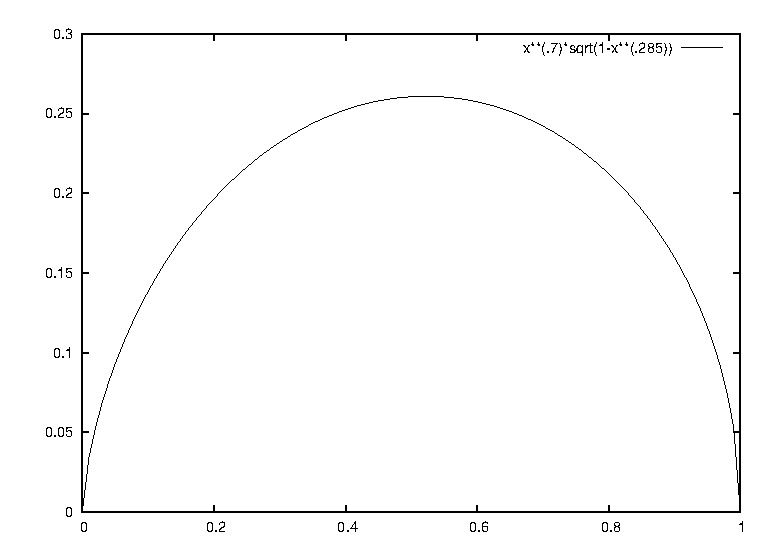
\includegraphics[width=450pt]{flux_vs_pressure.eps}
  \caption{質量流束と圧力比 (膨張比) の関係}
  \label{fig_flux_vs_pressure}
 \end{center}
\end{figure}

